\begin{statement}{3}
  In each part, use
  \[
    \Phi(x) = \prod_{i = 0}^n (x - t_i)
  \]
  to interpolate the given function using $n + 1$ evenly spaced
  nodes in the given interval. Plot each interpolant together with the exact function.
\end{statement}

\begin{solution}
  We are going to use the barycentric formula for the interpolating polynomial
  \lstinputlisting{scripts/algorithms/polyinterp.m}
\end{solution}

\begin{statement}{b}
  $f(x) = \tanh x$, $n = 2, 3, 4$, $x \in [1, 2]$.
\end{statement}

\begin{solution}
  With the following code
  \lstinputlisting{scripts/problems/problem-03-02.m}
  we obtain
  \begin{figure}[H]
    \centering
    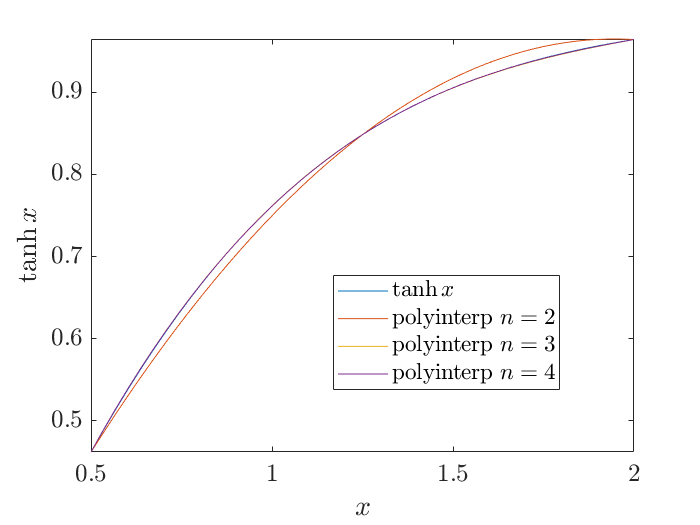
\includegraphics[scale=0.5]{graphics/plot-03-02.png}
    \caption{Polynomial interpolations of $\tanh x$ in $[0.5, 2]$}
  \end{figure}
\end{solution}

\begin{statement}{d}
  $f(x) = |x|$, $n = 2, 3, 4$, $x \in [-2, 1]$.
\end{statement}

\begin{solution}
  With the following code
  \lstinputlisting{scripts/problems/problem-03-04.m}
  we obtain
  \begin{figure}[H]
    \centering
    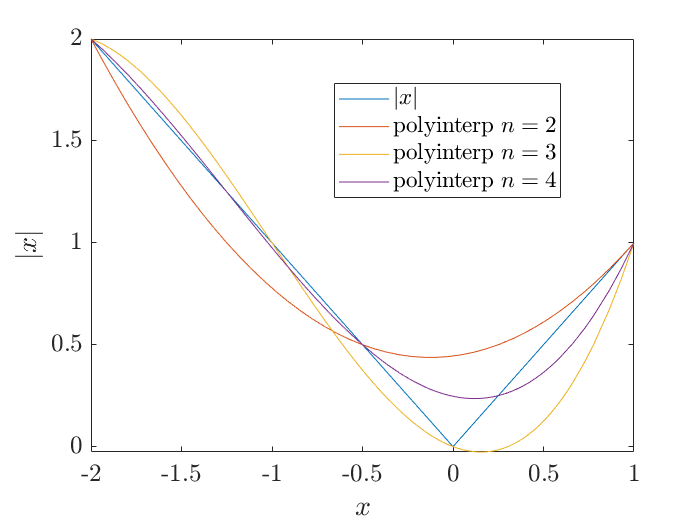
\includegraphics[scale=0.5]{graphics/plot-03-04.png}
    \caption{Polynomial interpolations of $|x|$ in $[-2, 1]$}
  \end{figure}
\end{solution}